%!TEX TS-program = xelatex
\documentclass[12pt, a4paper]{article} 
\usepackage{etex} % расширение классического tex в частности позволяет подгружать гораздо больше пакетов, чем мы и займёмся далее

%%%%%%%%%% Математика %%%%%%%%%%
\usepackage{amsmath,amsfonts,amssymb,amsthm,mathtools} 

%%%%%%%%%%%%%%%%%%%%%%%% Шрифты %%%%%%%%%%%%%%%%%%%%%%%%%%%%%%%%%
\usepackage{fontspec} % пакет для подгрузки шрифтов
\setmainfont{Arial} % задаёт основной шрифт документа
\defaultfontfeatures{Mapping=tex-text}
\newfontfamily{\cyrillicfonttt}{Arial} 
\newfontfamily{\cyrillicfont}{Arial} 
\newfontfamily{\cyrillicfontsf}{Arial}
\usepackage{polyglossia} % Пакет, который позволяет подгружать русские буквы
\setdefaultlanguage{russian} % Основной язык документа
\setotherlanguage{english} % Второстепенный язык документа

%%%%%%%%%% Работа с картинками %%%%%%%%%
\usepackage{graphicx} % Для вставки рисунков
\usepackage{graphics} 
\graphicspath{{images/}{pictures/}} % можно указать папки с картинками
\usepackage{wrapfig} % Обтекание рисунков и таблиц текстом
\usepackage{subfigure} % для создания нескольких рисунков внутри одного

\author{Кунакбаева Камила} 
\title{Задание 1 домашней 2}
\date{\today}

\begin{document} 

\maketitle

\begin{figure}
\begin{minipage}[h!]{0.3\linewidth}
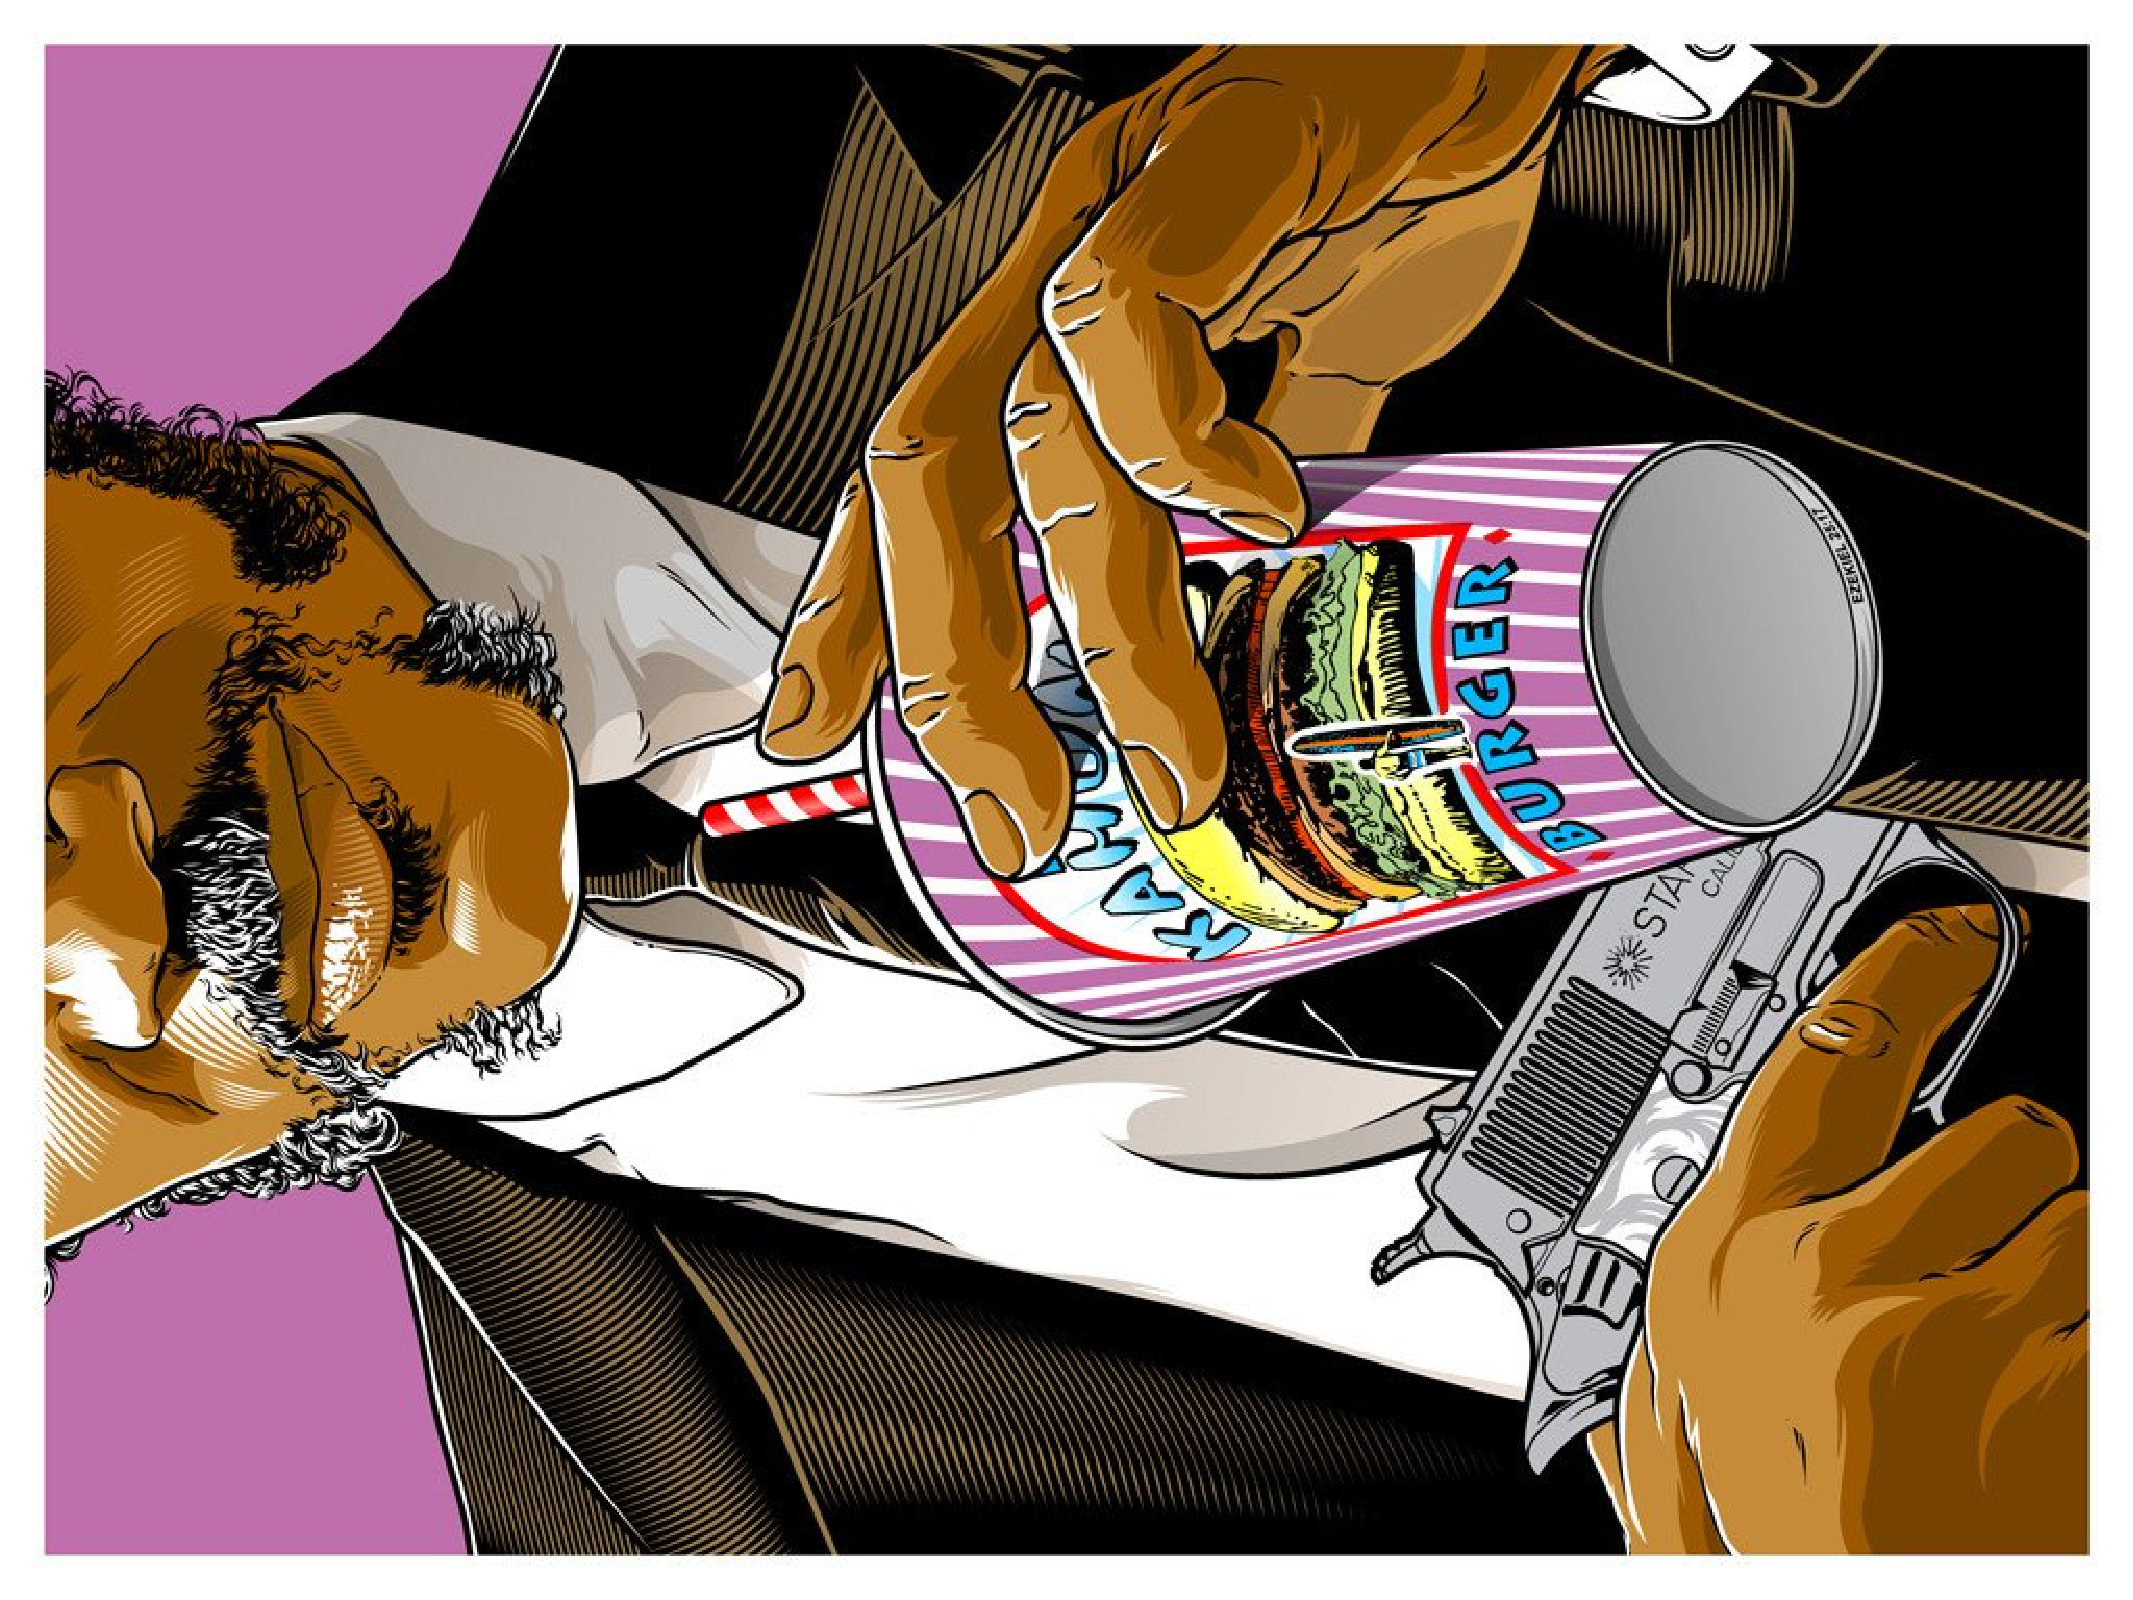
\includegraphics[height = 0.2\textheight,width=1.62\textwidth, angle=270]{pop1}
\end{minipage}
\hfil
\begin{minipage}[h!]{0.3\linewidth}

\includegraphics[width=1\textwidth, height = 0.32\textheight, angle=180]{pop2}
\end{minipage}
\hfil
\begin{minipage}[h!]{0.3\linewidth}

\includegraphics[width=1\textwidth, height = 0.32\textheight]{pop3}
\end{minipage}

\begin{minipage}[h!]{0.3\linewidth}
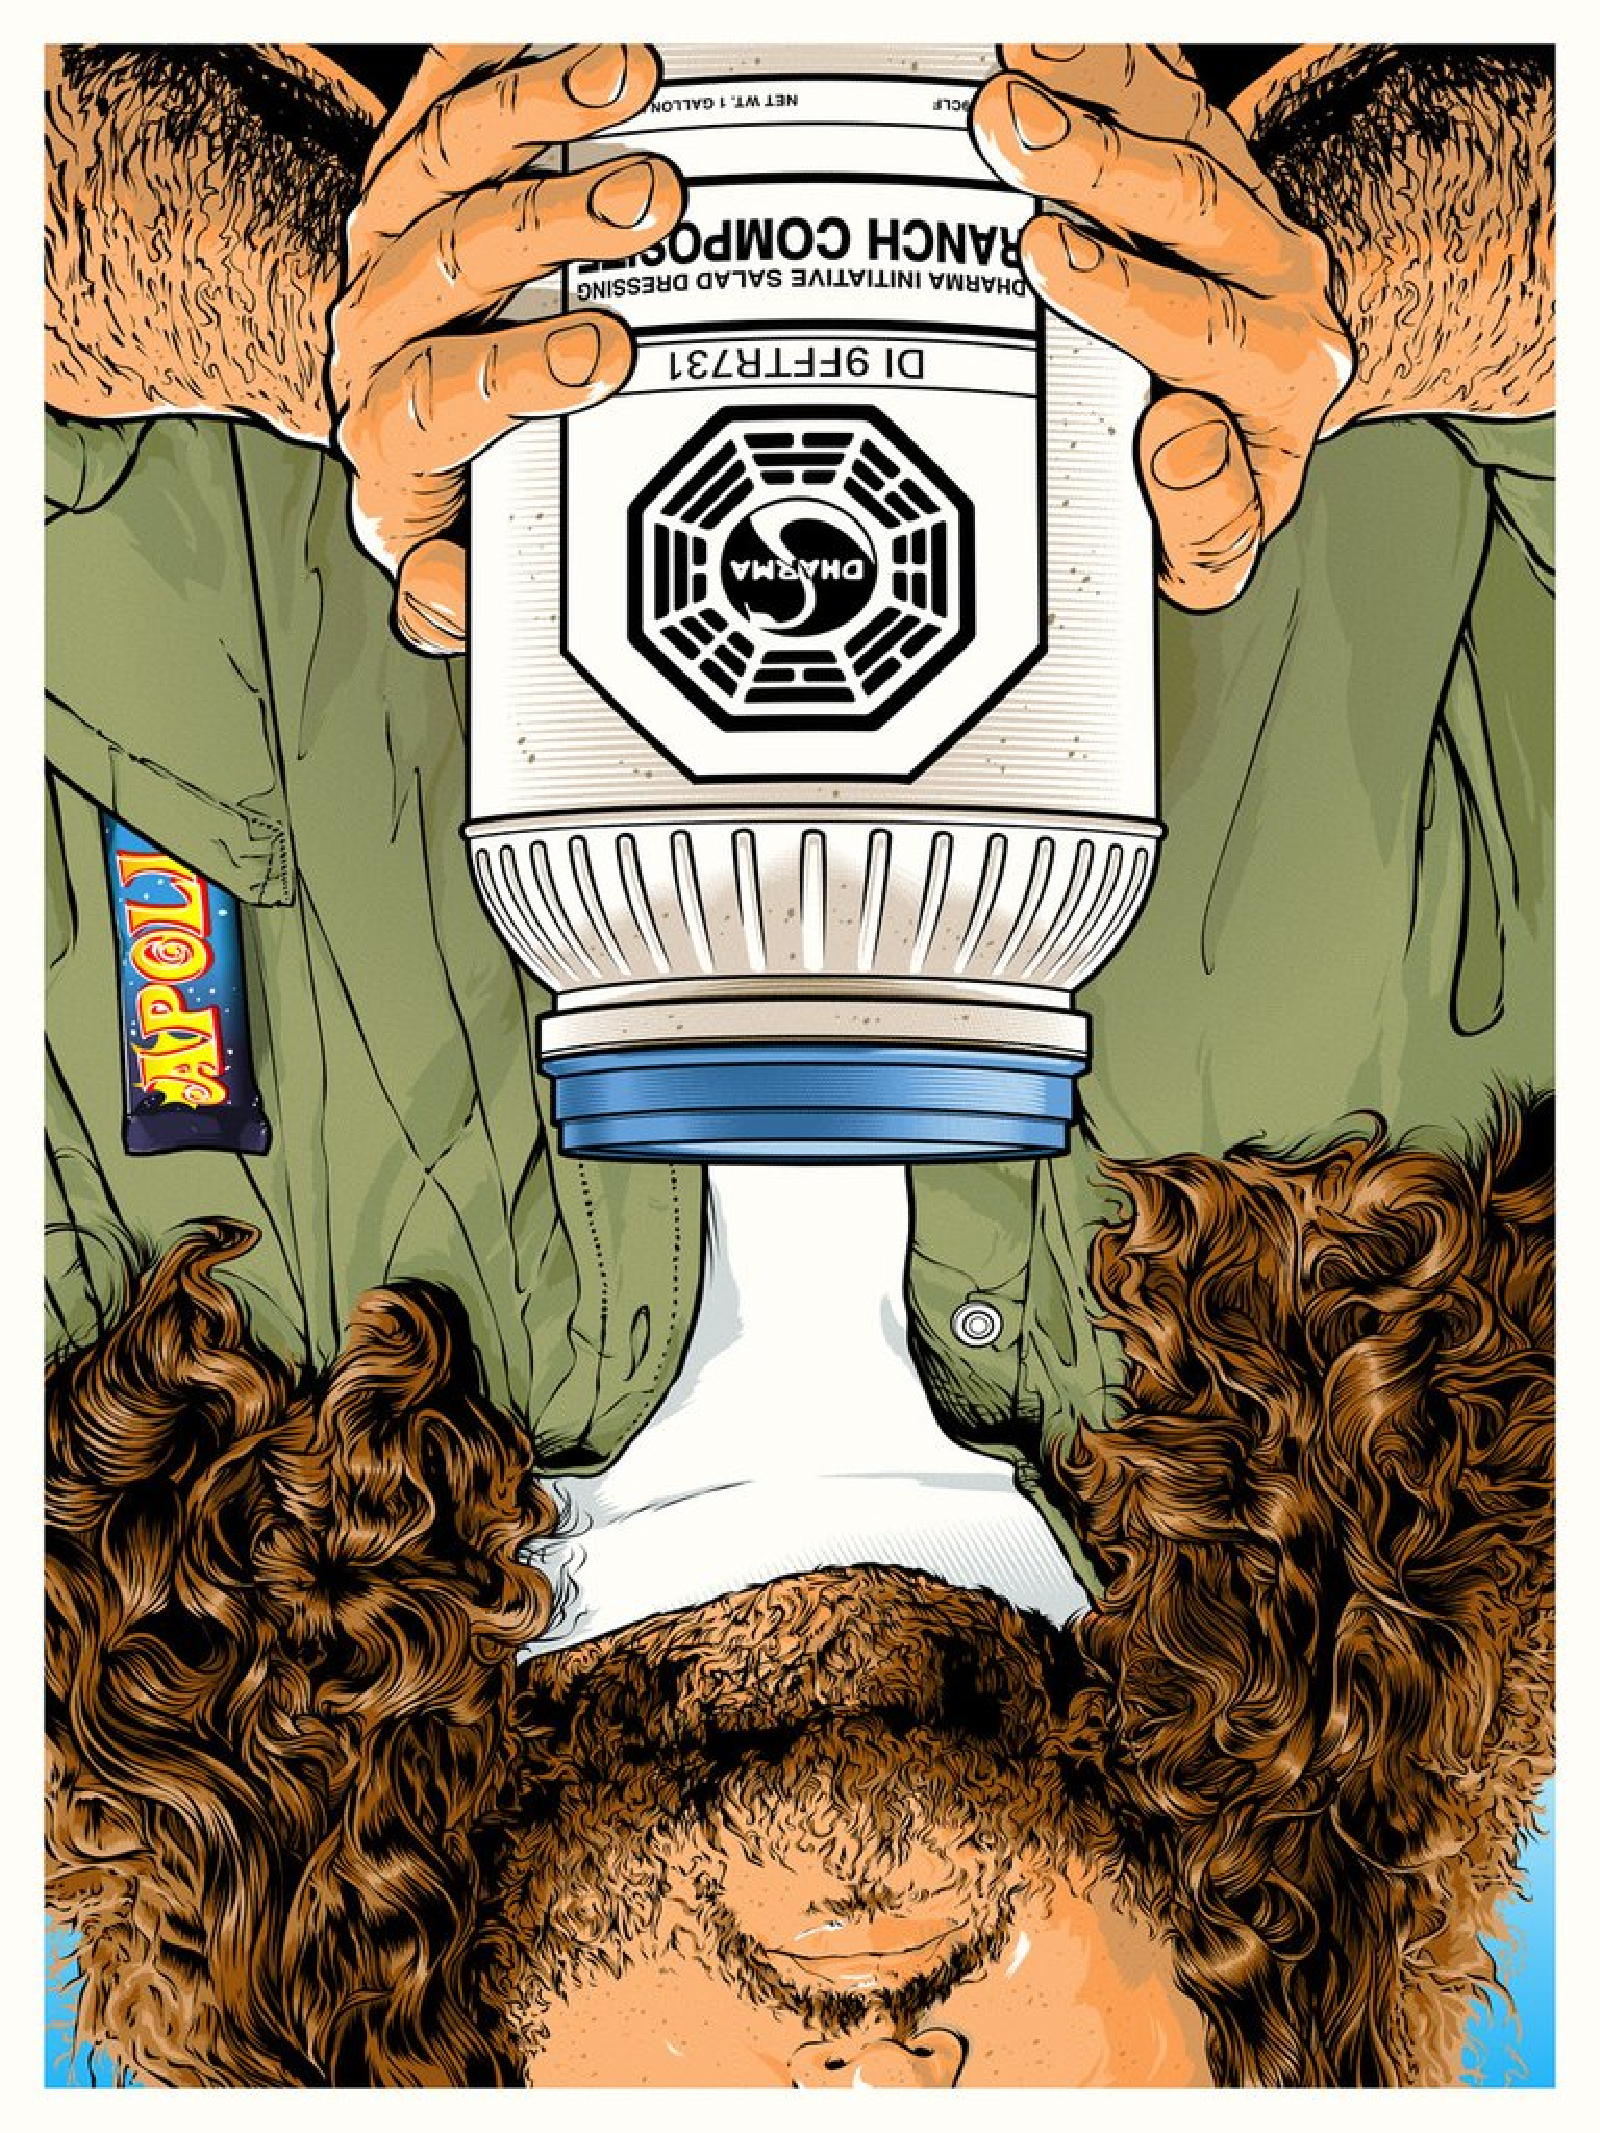
\includegraphics[width=1\textwidth, height = 0.32\textheight, angle=180]{pop10}
\end{minipage}
\hfil
\begin{minipage}[h!]{0.3\linewidth}
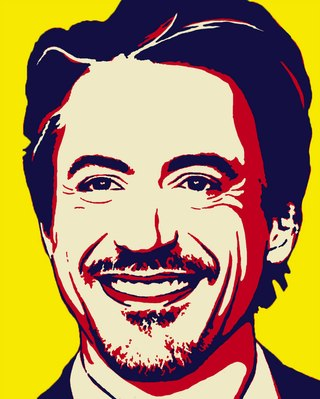
\includegraphics[width=1\textwidth, height = 0.32\textheight]{pop5}
\end{minipage}
\hfil
\begin{minipage}[h!]{0.3\linewidth}
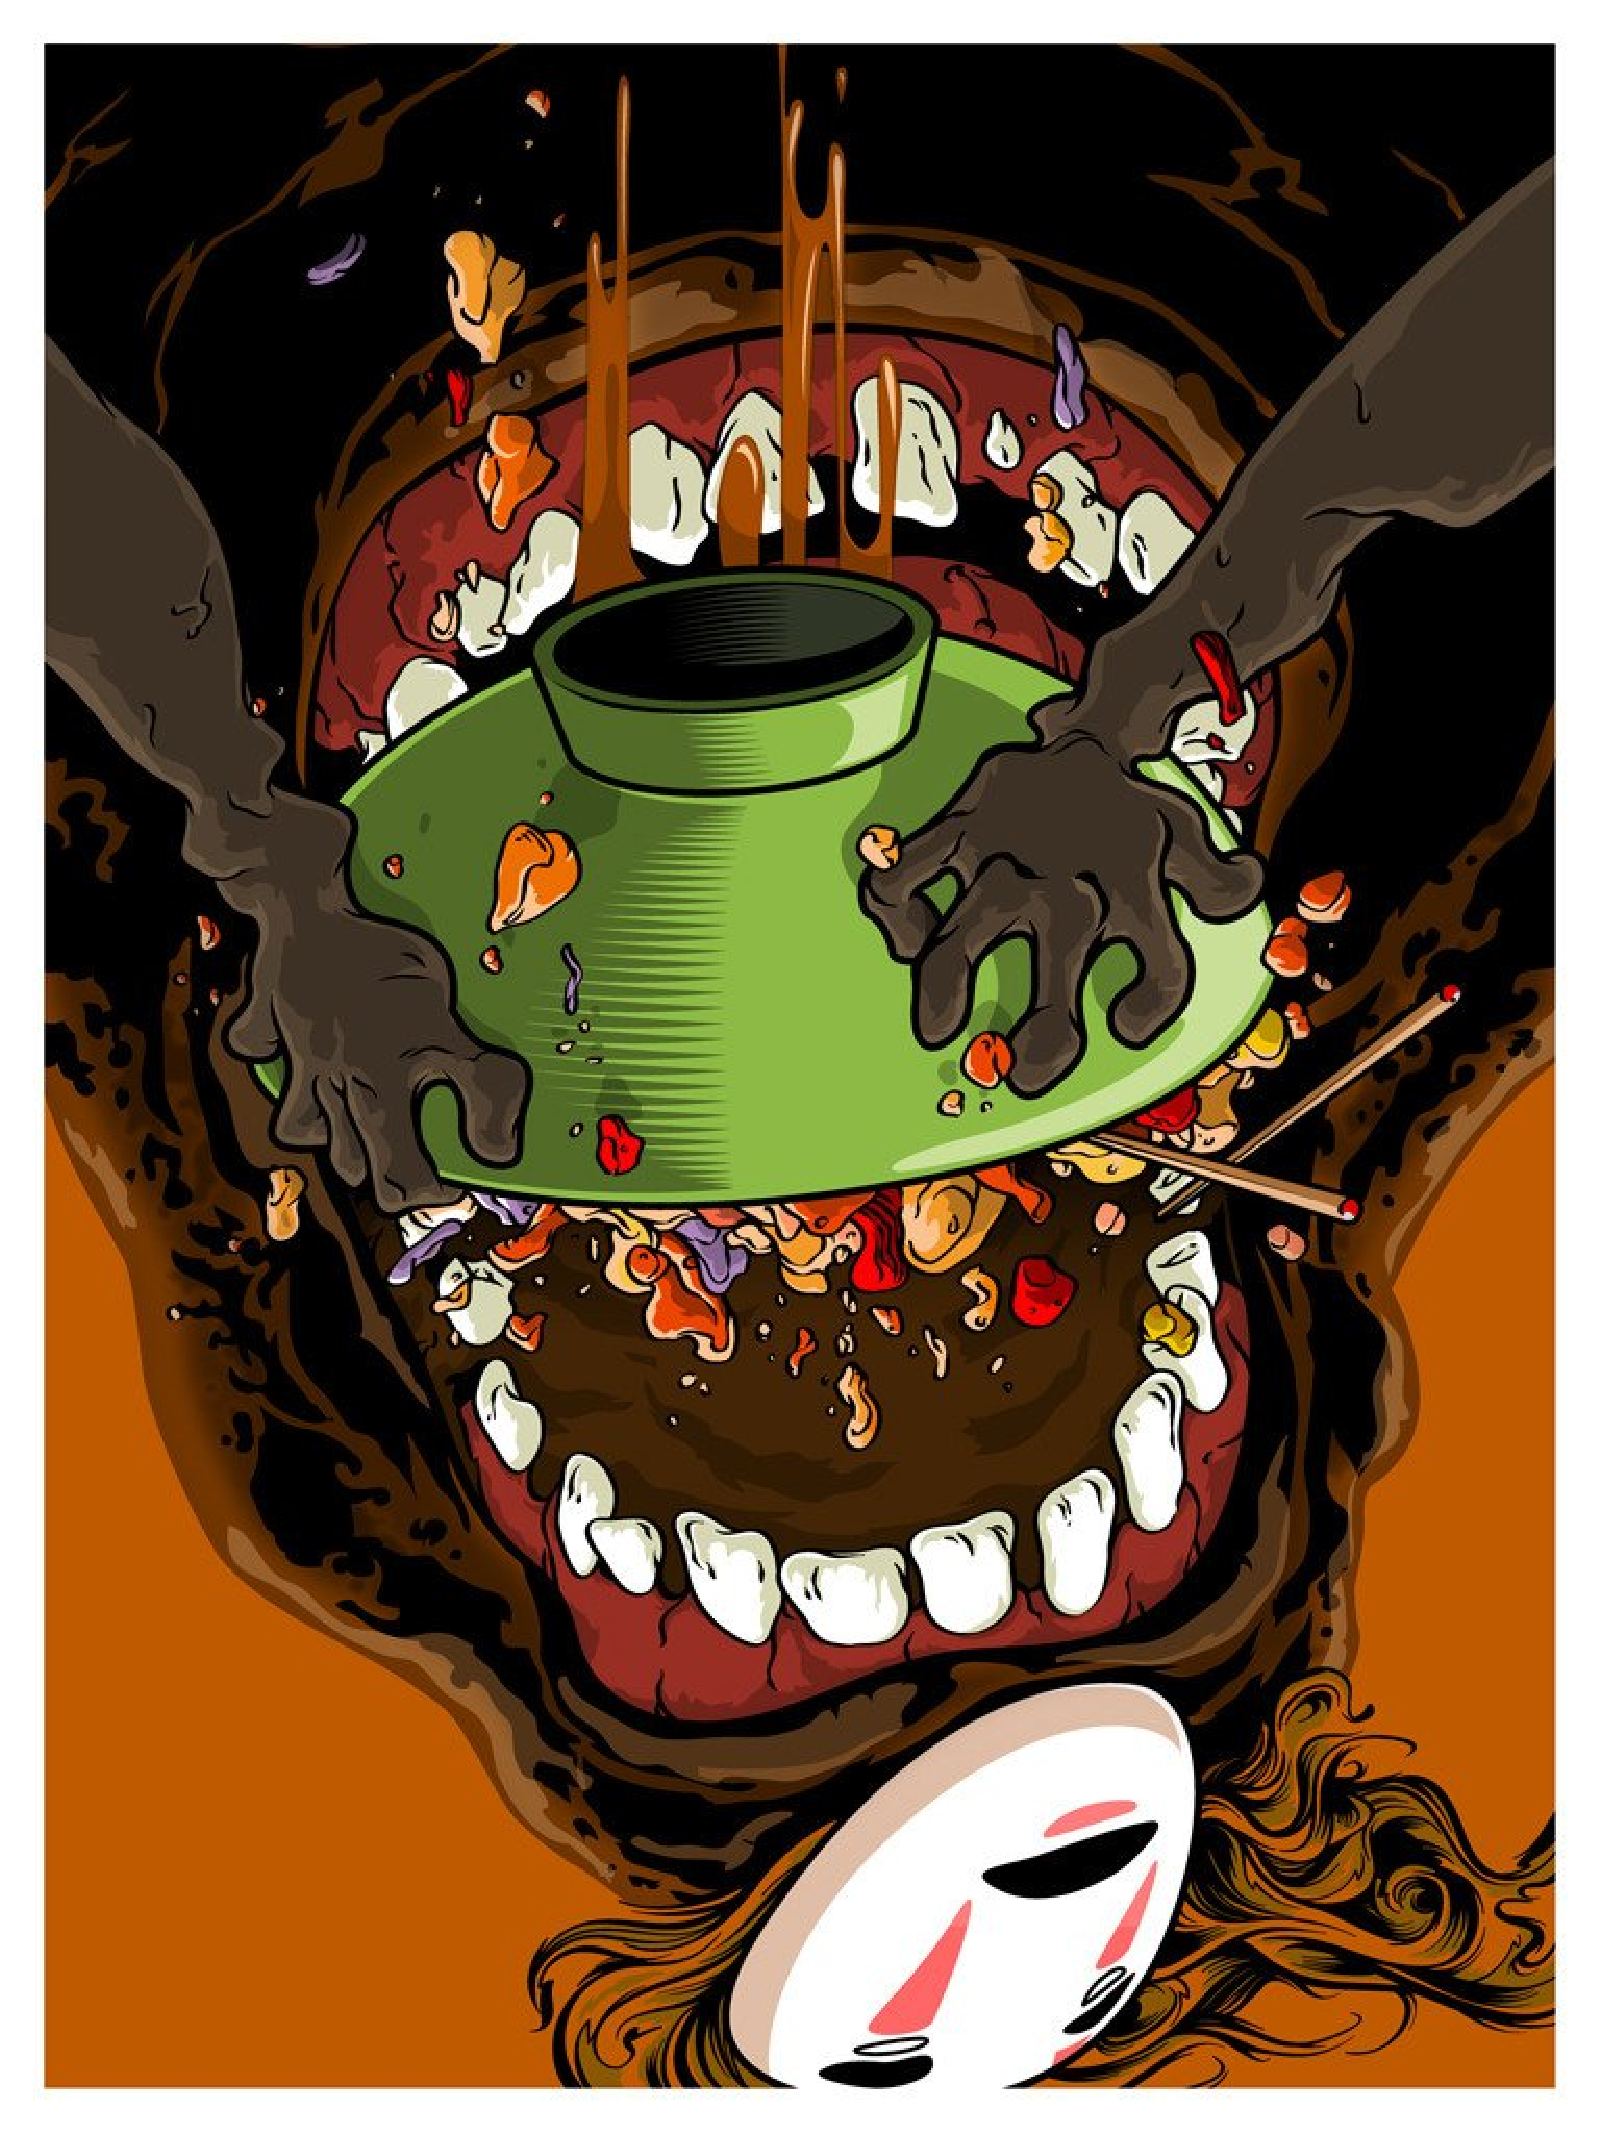
\includegraphics[width=1\textwidth, height = 0.32\textheight, angle=180]{pop6}
\end{minipage}
\end{figure}

\end{document}